\documentclass[10pt,aspectratio=169]{beamer}
\usepackage[utf8]{inputenc}
\usepackage{graphicx}
\usepackage{amsmath}
\usepackage{amssymb}
\usepackage{tikz}
\usetikzlibrary{shapes,arrows,positioning,3d,calc}
\usepackage{multicol}
\usepackage{booktabs}
\usepackage{xcolor}
\usepackage{siunitx}

% Color theme
\definecolor{primary}{RGB}{0,84,159}
\definecolor{secondary}{RGB}{142,186,229}
\definecolor{accent}{RGB}{227,114,34}
\definecolor{darkgray}{RGB}{50,50,50}
\setbeamercolor{structure}{fg=primary}
\setbeamercolor{title}{fg=white}
\setbeamercolor{frametitle}{fg=primary}
\setbeamercolor{block title}{fg=white,bg=primary}
\setbeamercolor{block body}{bg=secondary!20}
\setbeamercolor{alerted text}{fg=accent}
\setbeamercolor{normal text}{fg=darkgray}

% Beamer theme
\useinnertheme{rectangles}
\useoutertheme{miniframes}
\setbeamertemplate{navigation symbols}{}
\setbeamertemplate{footline}[frame number]

% Title page
\title{Robot Programming Languages and Systems}
\subtitle{Based on Chapters 12 \& 13 of Craig's Introduction to Robotics}
\author{Robotics Engineering}
\institute{Department of Mechanical Engineering}
\date{\today}

\begin{document}

% Title slide
\begin{frame}
\titlepage
\begin{tikzpicture}[remember picture,overlay]
\node[anchor=south east] at (current page.south east) {
\begin{tikzpicture}
\draw[primary,fill=primary!20] (0,0) circle (0.8);
\draw[primary,thick] (0,0.2) -- (0,0.6);
\draw[primary,thick] (-0.3,-0.3) -- (0.3,0.3);
\draw[primary,thick] (0.3,-0.3) -- (-0.3,0.3);
\end{tikzpicture}};
\end{tikzpicture}
\end{frame}

% Table of contents
\begin{frame}{Outline}
\tableofcontents
\end{frame}

\section{Chapter 12: Robot Programming Languages}

\begin{frame}{The Need for Specialized Robot Languages}
\begin{columns}[T]
\begin{column}{0.6\textwidth}
\begin{block}{Why Not General Programming Languages?}
\begin{itemize}
\item \textbf{Motion specification}: Natural description of positions and orientations
\item \textbf{Synchronization}: Coordination of multiple concurrent processes
\item \textbf{Sensor integration}: Easy interface with various sensor types
\item \textbf{World modeling}: Representation of objects and their relationships
\item \textbf{Exception handling}: Recovery from physical-world failures
\item \textbf{Real-time constraints}: Guaranteed timing for critical operations
\end{itemize}
\end{block}
\end{column}
\begin{column}{0.4\textwidth}
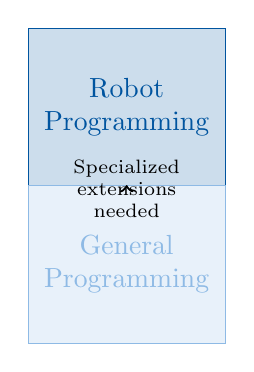
\begin{tikzpicture}[scale=0.8]
\node[draw,primary,fill=primary!20,minimum width=2.5cm,minimum height=2cm,align=center] (robot) at (0,0.5) {Robot\\Programming};
\node[draw,secondary,fill=secondary!20,minimum width=2.5cm,minimum height=2cm,align=center] (general) at (0,-2) {General\\Programming};
\draw[->,thick] (robot) -- (general);
\node[align=center,font=\scriptsize] at (0,-0.8) {Specialized\\extensions\\needed};
\end{tikzpicture}
\end{column}
\end{columns}
\end{frame}

\begin{frame}{Craig's Three-Generation Classification}
\begin{table}
\centering
\footnotesize
\begin{tabular}{p{0.25\textwidth}p{0.25\textwidth}p{0.25\textwidth}}
\toprule
\textbf{First Generation} & \textbf{Second Generation} & \textbf{Third Generation} \\
\midrule
Motion-oriented & Structured programming & Task-oriented \\
Explicit control & World modeling & Object-centered \\
Limited data types & Complex data structures & AI techniques \\
No sensor support & Sensor integration & Reasoning capabilities \\
No world model & Off-line programming & Automatic planning \\
\bottomrule
\end{tabular}
\end{table}

\begin{columns}[T]
\begin{column}{0.5\textwidth}
\begin{exampleblock}{First Generation Examples}
\begin{itemize}
\item \textbf{VAL (Unimation)}: First widely used language
\item \textbf{T3 (Cincinnati Milacron)}: Early industrial language
\item \textbf{ARLA (ASEA)}: For ASEA robots
\end{itemize}
\end{exampleblock}
\end{column}
\begin{column}{0.5\textwidth}
\begin{exampleblock}{Second/Third Generation Examples}
\begin{itemize}
\item \textbf{AML (IBM)}: Advanced features, strong typing
\item \textbf{RAIL (Automatix)}: Vision and force integration
\item \textbf{KAREL (Fanuc)}: Structured, teach pendant compatible
\end{itemize}
\end{exampleblock}
\end{column}
\end{columns}
\end{frame}

\begin{frame}{Key Language Features for Robotics}
\begin{columns}[T]
\begin{column}{0.5\textwidth}
\begin{block}{Motion Specification Features}
\begin{itemize}
\item \textbf{Joint-level motion}: MOVEJ (joint interpolated)
\item \textbf{Cartesian motion}: MOVEL (linear interpolation)
\item \textbf{Path specification}: Via points, blending
\item \textbf{Speed control}: Velocity, acceleration profiles
\item \textbf{Orientation control}: Euler angles, quaternions
\item \textbf{Frame specification}: Tool, user, world frames
\end{itemize}
\end{block}
\begin{alertblock}{Critical Features}
\begin{itemize}
\item \textbf{Synchronization}: WAIT, SIGNAL
\item \textbf{Concurrency}: Parallel execution
\item \textbf{Event handling}: Interrupts, exceptions
\item \textbf{Error recovery}: Retry mechanisms
\end{itemize}
\end{alertblock}
\end{column}
\begin{column}{0.5\textwidth}
\begin{block}{Sensor and I/O Features}
\begin{itemize}
\item \textbf{Digital I/O}: DOUT, DIN
\item \textbf{Analog I/O}: AOUT, AIN
\item \textbf{Force sensing}: READFORCE
\item \textbf{Vision}: FIND, LOCATE
\item \textbf{Position tracking}: POSITION
\end{itemize}
\end{block}
\begin{exampleblock}{Example Motion Commands (VAL)}
\ttfamily
MOVE P1\\
MOVES P2\\
APPRO P3, 50.0\\
DEPART 100.0
\end{exampleblock}
\end{column}
\end{columns}
\end{frame}

\begin{frame}{Detailed Analysis: VAL Language (Unimation)}
\begin{columns}[T]
\begin{column}{0.5\textwidth}
\begin{block}{VAL Key Features}
\begin{itemize}
\item Developed for PUMA robots
\item Teach pendant compatible
\item Two modes: Monitor and Program
\item Supports points, transformations
\item Real-time path modification
\item Force sensing integration
\end{itemize}
\end{block}
\begin{exampleblock}{Program Structure}
\ttfamily
.PROGRAM example()\\
\quad SPEED 100\\
\quad MOVES start\\
\quad OPENI\\
\quad APPRO part, 50\\
\quad CLOSEI\\
\quad DEPART 100\\
.END
\end{exampleblock}
\end{column}
\begin{column}{0.5\textwidth}
\begin{block}{VAL Data Types}
\begin{itemize}
\item \textbf{REAL}: Floating point numbers
\item \textbf{INTEGER}: Whole numbers
\item \textbf{STRING}: Text data
\item \textbf{TRANS}: Transformation matrices
\item \textbf{FRAME}: Position/orientation
\item \textbf{POINT}: 3D points
\end{itemize}
\end{block}
\begin{block}{Control Structures}
\begin{itemize}
\item IF...THEN...ELSE
\item WHILE...DO
\item FOR...TO
\item REPEAT...UNTIL
\item CALL: Subroutine calls
\end{itemize}
\end{block}
\end{column}
\end{columns}
\end{frame}

\begin{frame}{Detailed Analysis: AML Language (IBM)}
\begin{columns}[T]
\begin{column}{0.6\textwidth}
\begin{block}{AML Design Principles}
\begin{itemize}
\item \textbf{Strong typing}: Compile-time type checking
\item \textbf{Modularity}: Separate compilation units
\item \textbf{Portability}: Multiple robot support
\item \textbf{Real-time}: Deterministic execution
\item \textbf{Safety}: Built-in protection mechanisms
\end{itemize}
\end{block}
\begin{alertblock}{Advanced Features}
\begin{itemize}
\item \textbf{Data abstraction}: User-defined types
\item \textbf{Exception handling}: Structured error recovery
\item \textbf{Concurrent processes}: Parallel execution
\item \textbf{World modeling}: Object relationships
\item \textbf{Off-line programming}: Simulation support
\end{itemize}
\end{alertblock}
\end{column}
\begin{column}{0.4\textwidth}
\begin{exampleblock}{AML Example}
\ttfamily
PROCEDURE assemble()\\
BEGIN\\
\quad MOVE arm TO approach;\\
\quad GRASP part WITH force := 20.0;\\
\quad MOVE arm TO fixture;\\
\quad INSERT part INTO hole;\\
\quad RELEASE;\\
END assemble;
\end{exampleblock}
\end{column}
\end{columns}

\begin{block}{AML vs VAL Comparison}
\begin{itemize}
\item \textbf{AML}: Strongly typed, structured, modular
\item \textbf{VAL}: Weakly typed, interpretive, simple
\item \textbf{AML}: Better for complex applications
\item \textbf{VAL}: Easier for simple tasks
\end{itemize}
\end{block}
\end{frame}

\begin{frame}{Modern Robot Programming Languages}
\begin{columns}[T]
\begin{column}{0.5\textwidth}
\begin{block}{Industrial Languages}
\begin{itemize}
\item \textbf{RAPID (ABB)}: Structured, task-based
\item \textbf{KAREL (Fanuc)}: Pascal-like, teach pendant
\item \textbf{IRL (KUKA)}: C-like syntax, powerful
\item \textbf{INFORM (Kawasaki)}: Flexible, comprehensive
\item \textbf{AS (Mitsubishi)}: Simple, intuitive
\end{itemize}
\end{block}
\begin{alertblock}{Research Languages}
\begin{itemize}
\item \textbf{SMALLTALK}: Object-oriented, interactive
\item \textbf{LISP}: Symbolic processing, AI
\item \textbf{PROLOG}: Logic programming, planning
\end{itemize}
\end{alertblock}
\end{column}
\begin{column}{0.5\textwidth}
\begin{block}{Programming Language Trends}
\begin{table}
\centering
\scriptsize
\begin{tabular}{p{0.45\textwidth}p{0.45\textwidth}}
\toprule
\textbf{Traditional} & \textbf{Modern} \\
\midrule
Vendor-specific & Cross-platform \\
Teach pendant & PC-based \\
Textual & Graphical \\
Sequential & Concurrent \\
Limited types & Rich types \\
\bottomrule
\end{tabular}
\end{table}
\end{block}
\begin{exampleblock}{RAPID Example (ABB)}
\ttfamily
PROC main()\\
\quad MoveJ pHome, v1000, fine, tool0;\\
\quad MoveL pPick, v500, fine, tool0;\\
\quad SetDO gripper, 1;\\
\quad MoveL pPlace, v500, fine, tool0;\\
\quad SetDO gripper, 0;\\
ENDPROC
\end{exampleblock}
\end{column}
\end{columns}
\end{frame}

\section{Chapter 13: Off-line Programming Systems}

\begin{frame}{Definition and Motivation for Off-line Programming}
\begin{columns}[T]
\begin{column}{0.6\textwidth}
\begin{block}{What is Off-line Programming?}
\textbf{Off-line Programming (OLP)}: Creating robot programs without using the actual robot, typically using computer simulation.
\end{block}
\begin{alertblock}{Key Motivations}
\begin{itemize}
\item \textbf{Reduced downtime}: Program while production runs
\item \textbf{Complex tasks}: Handle tasks too complex for teach pendant
\item \textbf{Safety}: Test dangerous operations virtually
\item \textbf{CAD integration}: Direct use of design data
\item \textbf{Optimization}: Multiple iterations without robot time
\item \textbf{Documentation}: Automatic program documentation
\end{itemize}
\end{alertblock}
\end{column}
\begin{column}{0.4\textwidth}
\begin{center}
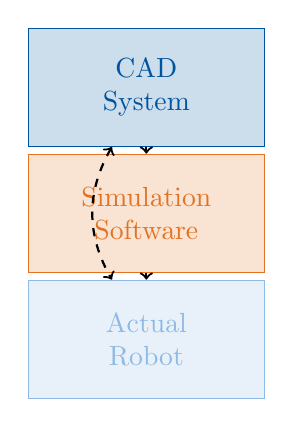
\begin{tikzpicture}[scale=0.8]
\node[draw,primary,fill=primary!20,minimum width=3cm,minimum height=1.5cm,align=center] (cad) at (0,2) {CAD\\System};
\node[draw,accent,fill=accent!20,minimum width=3cm,minimum height=1.5cm,align=center] (sim) at (0,0) {Simulation\\Software};
\node[draw,secondary,fill=secondary!20,minimum width=3cm,minimum height=1.5cm,align=center] (robot) at (0,-2) {Actual\\Robot};
\draw[->,thick] (cad) -- (sim);
\draw[->,thick] (sim) -- (robot);
\draw[<->,thick,dashed] (cad) to[bend right=30] (robot);
\end{tikzpicture}
\end{center}
\end{column}
\end{columns}
\end{frame}

\begin{frame}{OLP System Architecture}
\begin{columns}[T]
\begin{column}{0.5\textwidth}
\begin{block}{Core Components}
\begin{enumerate}
\item \textbf{CAD Interface}: Import part geometry
\item \textbf{Robot Library}: Kinematic models
\item \textbf{Workspace Modeling}: Environment definition
\item \textbf{Path Planning}: Motion generation
\item \textbf{Collision Detection}: Interference checking
\item \textbf{Program Generator}: Code output
\item \textbf{Simulation Engine}: Virtual execution
\item \textbf{Post-processor}: Robot-specific adaptation
\end{enumerate}
\end{block}
\end{column}
\begin{column}{0.5\textwidth}
\begin{center}
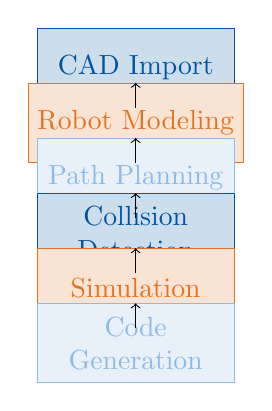
\begin{tikzpicture}[scale=0.7]
\node[draw,primary,fill=primary!20,minimum width=2.5cm,minimum height=1cm,align=center] (cad) at (0,4) {CAD Import};
\node[draw,accent,fill=accent!20,minimum width=2.5cm,minimum height=1cm,align=center] (model) at (0,3) {Robot Modeling};
\node[draw,secondary,fill=secondary!20,minimum width=2.5cm,minimum height=1cm,align=center] (path) at (0,2) {Path Planning};
\node[draw,primary,fill=primary!20,minimum width=2.5cm,minimum height=1cm,align=center] (coll) at (0,1) {Collision\\Detection};
\node[draw,accent,fill=accent!20,minimum width=2.5cm,minimum height=1cm,align=center] (sim) at (0,0) {Simulation};
\node[draw,secondary,fill=secondary!20,minimum width=2.5cm,minimum height=1cm,align=center] (code) at (0,-1) {Code\\Generation};
\draw[->] (cad) -- (model);
\draw[->] (model) -- (path);
\draw[->] (path) -- (coll);
\draw[->] (coll) -- (sim);
\draw[->] (sim) -- (code);
\end{tikzpicture}
\end{center}
\end{column}
\end{columns}

\vspace{0.5cm}
\begin{alertblock}{Data Flow in OLP Systems}
CAD Models $\rightarrow$ Robot Library $\rightarrow$ Task Definition $\rightarrow$ Path Planning $\rightarrow$ Simulation $\rightarrow$ Program Generation $\rightarrow$ Robot Controller
\end{alertblock}
\end{frame}

\begin{frame}{Robot Modeling for OLP Systems}
\begin{columns}[T]
\begin{column}{0.6\textwidth}
\begin{block}{Kinematic Modeling}
\begin{itemize}
\item \textbf{DH parameters}: Standard representation
\item \textbf{Forward kinematics}: Position from joint angles
\item \textbf{Inverse kinematics}: Joint angles from position
\item \textbf{Workspace analysis}: Reachable volume calculation
\item \textbf{Singularity detection}: Problematic configurations
\end{itemize}
\end{block}
\begin{alertblock}{Dynamic Modeling (Advanced)}
\begin{itemize}
\item \textbf{Mass properties}: Mass, center of gravity
\item \textbf{Inertia tensors}: Rotational inertia
\item \textbf{Motor characteristics}: Torque, speed limits
\item \textbf{Friction models}: Static and dynamic friction
\end{itemize}
\end{alertblock}
\end{column}
\begin{column}{0.4\textwidth}
\begin{center}
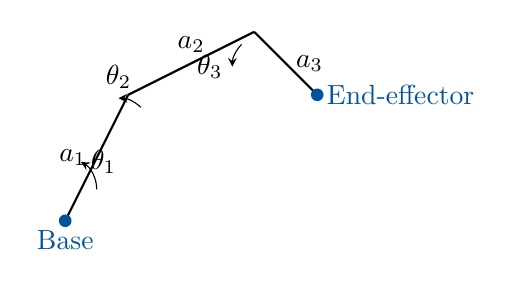
\begin{tikzpicture}[scale=0.8]
\coordinate (O) at (0,0);
\coordinate (A) at (1,2);
\coordinate (B) at (3,3);
\coordinate (C) at (4,2);
\draw[thick] (O) -- (A) node[midway,left]{$a_1$};
\draw[thick] (A) -- (B) node[midway,above]{$a_2$};
\draw[thick] (B) -- (C) node[midway,right]{$a_3$};
\draw[->,>=stealth] (0.5,0.5) arc (0:60:0.5) node[right]{$\theta_1$};
\draw[->,>=stealth] (1.2,1.8) arc (45:90:0.5) node[above]{$\theta_2$};
\draw[->,>=stealth] (2.8,2.8) arc (135:180:0.5) node[left]{$\theta_3$};
\fill[primary] (O) circle (0.1) node[below]{Base};
\fill[primary] (C) circle (0.1) node[right]{End-effector};
\end{tikzpicture}
\end{center}
\end{column}
\end{columns}

\begin{block}{Model Accuracy Requirements}
\begin{itemize}
\item \textbf{Position accuracy}: $\pm 1$ mm typically needed
\item \textbf{Orientation accuracy}: $\pm 0.1$ degrees
\item \textbf{Cycle time}: Within 5\% of actual
\item \textbf{Workspace}: Within 95\% match to real robot
\end{itemize}
\end{block}
\end{frame}

\begin{frame}{Workspace Modeling and Environment Definition}
\begin{columns}[T]
\begin{column}{0.5\textwidth}
\begin{block}{Environmental Components}
\begin{itemize}
\item \textbf{Fixtures}: Clamps, vises, positioning devices
\item \textbf{Obstacles}: Safety fences, other equipment
\item \textbf{Conveyors}: Moving components
\item \textbf{Tools}: End-effectors, grippers
\item \textbf{Workpieces}: Parts to be processed
\item \textbf{Auxiliary equipment}: Welding guns, dispensers
\end{itemize}
\end{block}
\begin{alertblock}{Model Sources}
\begin{itemize}
\item \textbf{CAD files}: STEP, IGES, SAT formats
\item \textbf{3D scanning}: Point cloud data
\item \textbf{Manual creation}: Primitive shapes
\item \textbf{Library components}: Standard items
\end{itemize}
\end{alertblock}
\end{column}
\begin{column}{0.5\textwidth}
\begin{center}
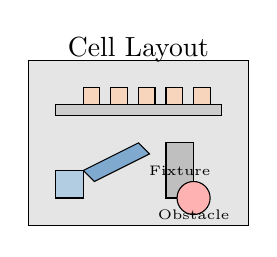
\begin{tikzpicture}[scale=0.7]
\draw[fill=gray!20] (0,0) rectangle (4,3);
\node at (2,3.2) {Cell Layout};
\draw[fill=primary!30] (0.5,0.5) rectangle (1,1);
\draw[fill=primary!50] (1,1) -- (2,1.5) -- (2.2,1.3) -- (1.2,0.8) -- cycle;
\draw[fill=gray!50] (2.5,0.5) rectangle (3,1.5);
\node[font=\tiny] at (2.75,1) {Fixture};
\draw[fill=gray!40] (0.5,2) rectangle (3.5,2.2);
\foreach \x in {1,1.5,2,2.5,3} {
    \draw[fill=accent!30] (\x,2.2) rectangle (\x+0.3,2.5);
}
\draw[fill=red!30] (3,0.5) circle (0.3);
\node[font=\tiny] at (3,0.2) {Obstacle};
\end{tikzpicture}
\end{center}
\end{column}
\end{columns}

\vspace{0.5cm}
\begin{block}{Coordinate System Management}
\begin{itemize}
\item \textbf{World coordinate system}: Global reference
\item \textbf{Robot base frame}: Robot reference point
\item \textbf{Tool frame}: End-effector tip
\item \textbf{User frames}: Workpiece-specific coordinates
\item \textbf{Calibration frames}: Alignment references
\end{itemize}
\end{block}
\end{frame}

\begin{frame}{Path Planning in OLP Systems}
\begin{columns}[T]
\begin{column}{0.5\textwidth}
\begin{block}{Path Planning Methods}
\begin{enumerate}
\item \textbf{Manual teaching}: Virtual teach pendant
\item \textbf{Automatic generation}: From CAD features
\item \textbf{Template-based}: Reusable patterns
\item \textbf{Optimization-based}: Performance criteria
\item \textbf{Lead-through}: Virtual guiding
\end{enumerate}
\end{block}
\begin{alertblock}{Path Types}
\begin{itemize}
\item \textbf{Joint motion}: Fastest, but unpredictable path
\item \textbf{Linear motion}: Straight line in Cartesian space
\item \textbf{Circular motion}: Arc segments
\item \textbf{Spline motion}: Smooth curves
\end{itemize}
\end{alertblock}
\end{column}
\begin{column}{0.5\textwidth}
\begin{center}
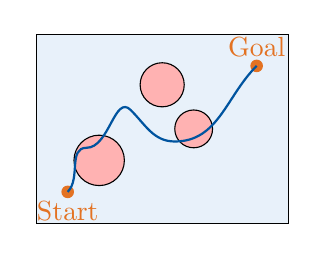
\begin{tikzpicture}[scale=0.8]
\draw[fill=secondary!20] (0,0) rectangle (4,3);
\fill[accent] (0.5,0.5) circle (0.1) node[below]{Start};
\fill[accent] (3.5,2.5) circle (0.1) node[above]{Goal};
\draw[fill=red!30] (1,1) circle (0.4);
\draw[fill=red!30] (2.5,1.5) circle (0.3);
\draw[fill=red!30] (2,2.2) circle (0.35);
\draw[primary,thick] (0.5,0.5) to[out=45,in=180] (0.8,1.2) 
                     to[out=0,in=135] (1.5,1.8)
                     to[out=315,in=180] (2.2,1.3)
                     to[out=0,in=225] (3.5,2.5);
\end{tikzpicture}
\end{center}
\end{column}
\end{columns}

\vspace{0.5cm}
\begin{block}{Path Optimization Criteria}
\begin{itemize}
\item \textbf{Time minimization}: Shortest cycle time
\item \textbf{Energy efficiency}: Minimum power consumption
\item \textbf{Jerk limitation}: Smooth acceleration changes
\item \textbf{Collision avoidance}: Safe clearances
\item \textbf{Singularity avoidance}: Stay away from singularities
\end{itemize}
\end{block}
\end{frame}

\begin{frame}{Collision Detection and Avoidance}
\begin{columns}[T]
\begin{column}{0.6\textwidth}
\begin{block}{Detection Methods}
\begin{enumerate}
\item \textbf{Bounding volumes}: Spheres, boxes, cylinders
\item \textbf{Hierarchical methods}: Octrees, BSP trees
\item \textbf{Polygon testing}: Triangle intersection
\item \textbf{Distance computation}: Minimum separation
\end{enumerate}
\end{block}
\begin{alertblock}{Real-time Considerations}
\begin{itemize}
\item \textbf{Update rate}: 30-60 Hz for simulation
\item \textbf{Accuracy vs speed trade-off}
\item \textbf{Multiple collision pairs}
\item \textbf{Moving obstacles}
\end{itemize}
\end{alertblock}
\end{column}
\begin{column}{0.4\textwidth}
\begin{center}
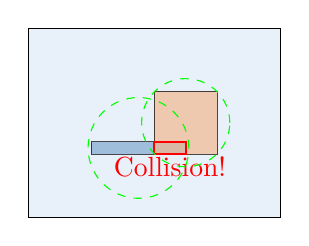
\begin{tikzpicture}[scale=0.8]
\draw[fill=secondary!20] (0,0) rectangle (4,3);
\draw[fill=primary!50,opacity=0.7] (1,1) rectangle (2.5,1.2);
\draw[fill=accent!50,opacity=0.7] (2,1) rectangle (3,2);
\draw[red,thick] (2,1) rectangle (2.5,1.2);
\node[red] at (2.25,0.8) {Collision!};
\draw[green,dashed] (1.75,1.1) circle (0.8);
\draw[green,dashed] (2.5,1.5) circle (0.7);
\end{tikzpicture}
\end{center}
\end{column}
\end{columns}

\vspace{0.5cm}
\begin{block}{Clearance Checking Levels}
\begin{table}
\centering
\scriptsize
\begin{tabular}{p{0.25\textwidth}p{0.25\textwidth}p{0.25\textwidth}}
\toprule
\textbf{Level} & \textbf{Method} & \textbf{Accuracy} \\
\midrule
\textbf{Coarse} & Bounding boxes & Fast, approximate \\
\textbf{Medium} & Convex hulls & Balance \\
\textbf{Fine} & Polygon exact & Slow, exact \\
\bottomrule
\end{tabular}
\end{table}
\end{block}
\end{frame}

\begin{frame}{Program Generation and Post-processing}
\begin{columns}[T]
\begin{column}{0.5\textwidth}
\begin{block}{Post-processing Tasks}
\begin{enumerate}
\item \textbf{Kinematic conversion}: Simulation to robot coordinates
\item \textbf{Speed adaptation}: Velocity profile generation
\item \textbf{Coordinate transformation}: Frame conversions
\item \textbf{Collision avoidance}: Adding safe points
\item \textbf{Error handling}: Inserting recovery routines
\item \textbf{Comments}: Adding documentation
\end{enumerate}
\end{block}
\begin{alertblock}{Robot-Specific Adaptations}
\begin{itemize}
\item \textbf{Joint limits}: Respecting mechanical constraints
\item \textbf{Singularities}: Avoiding problematic poses
\item \textbf{Controller capabilities}: Using supported features
\item \textbf{Communication protocol}: Proper format
\end{itemize}
\end{alertblock}
\end{column}
\begin{column}{0.5\textwidth}
\begin{block}{Code Generation Process}
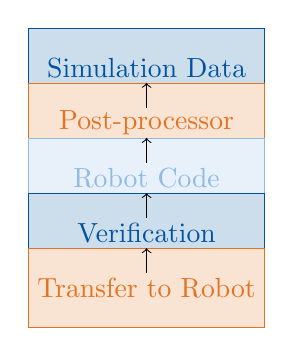
\begin{tikzpicture}[scale=0.7]
\node[draw,primary,fill=primary!20,minimum width=3cm,minimum height=1cm,align=center] (sim) at (0,3) {Simulation Data};
\node[draw,accent,fill=accent!20,minimum width=3cm,minimum height=1cm,align=center] (post) at (0,2) {Post-processor};
\node[draw,secondary,fill=secondary!20,minimum width=3cm,minimum height=1cm,align=center] (code) at (0,1) {Robot Code};
\node[draw,primary,fill=primary!20,minimum width=3cm,minimum height=1cm,align=center] (verify) at (0,0) {Verification};
\node[draw,accent,fill=accent!20,minimum width=3cm,minimum height=1cm,align=center] (transfer) at (0,-1) {Transfer to Robot};
\draw[->] (sim) -- (post);
\draw[->] (post) -- (code);
\draw[->] (code) -- (verify);
\draw[->] (verify) -- (transfer);
\end{tikzpicture}
\end{block}
\end{column}
\end{columns}

\vspace{0.5cm}
\begin{exampleblock}{Generated RAPID Code Example}
\ttfamily
! Generated by OLP System v2.1\\
! Part: Assembly\_Plate\_A\\
! Date: 2024-01-15\\
\\
PROC Main()\\
\quad MoveJ Home,v1000,z50,tool0;\\
\quad MoveJ Approach\_P1,v500,fine,tool0;\\
\quad MoveL Pick\_Position,v200,fine,tool0;\\
\quad SetDO Gripper,1;\\
\quad WaitTime 0.5;\\
\quad MoveL Approach\_P1,v200,fine,tool0;\\
ENDPROC
\end{exampleblock}
\end{frame}

\begin{frame}{Calibration and Accuracy Issues}
\begin{columns}[T]
\begin{column}{0.6\textwidth}
\begin{block}{Sources of Error}
\begin{itemize}
\item \textbf{Model inaccuracies}: CAD vs actual dimensions
\item \textbf{Robot calibration}: Kinematic parameter errors
\item \textbf{Workpiece positioning}: Fixture variations
\item \textbf{Tool definition}: TCP measurement errors
\item \textbf{Thermal effects}: Expansion/contraction
\end{itemize}
\end{block}
\begin{alertblock}{Calibration Methods}
\begin{enumerate}
\item \textbf{Manual measurement}: Using calibration tools
\item \textbf{Vision systems}: Camera-based alignment
\item \textbf{Probe-based}: Touch probe measurements
\item \textbf{Laser tracking}: High-precision measurement
\item \textbf{Automated calibration}: Self-calibration routines
\end{enumerate}
\end{alertblock}
\end{column}
\begin{column}{0.4\textwidth}
\begin{center}
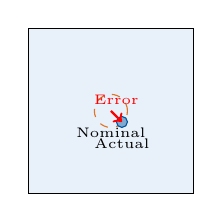
\begin{tikzpicture}[scale=0.7]
\draw[fill=secondary!20] (0,0) rectangle (3,3);
\draw[accent,dashed] (1.5,1.5) circle (0.3);
\node[font=\tiny] at (1.5,1.1) {Nominal};
\draw[primary,fill=primary!50] (1.7,1.3) circle (0.1);
\node[font=\tiny] at (1.7,0.9) {Actual};
\draw[red,thick,->] (1.5,1.5) -- (1.7,1.3);
\node[red,font=\tiny] at (1.6,1.7) {Error};
\end{tikzpicture}
\end{center}
\end{column}
\end{columns}

\vspace{0.5cm}
\begin{block}{Typical Accuracy Requirements}
\begin{table}
\centering
\scriptsize
\begin{tabular}{p{0.3\textwidth}p{0.3\textwidth}p{0.3\textwidth}}
\toprule
\textbf{Application} & \textbf{Position Accuracy} & \textbf{Orientation Accuracy} \\
\midrule
\textbf{Material handling} & $\pm 5$ mm & $\pm 2^\circ$ \\
\textbf{Spot welding} & $\pm 1$ mm & $\pm 1^\circ$ \\
\textbf{Arc welding} & $\pm 0.5$ mm & $\pm 0.5^\circ$ \\
\textbf{Assembly} & $\pm 0.1$ mm & $\pm 0.1^\circ$ \\
\bottomrule
\end{tabular}
\end{table}
\end{block}
\end{frame}

\begin{frame}{Commercial OLP Systems Overview}
\begin{columns}[T]
\begin{column}{0.5\textwidth}
\begin{block}{Leading Commercial Systems}
\begin{itemize}
\item \textbf{Delmia (Dassault)}: CATIA integration
\item \textbf{RoboGuide (Fanuc)}: Fanuc-specific
\item \textbf{RobotStudio (ABB)}: ABB-specific
\item \textbf{KUKA.Sim (KUKA)}: KUKA-specific
\item \textbf{Octopuz}: Multi-vendor support
\item \textbf{RoboDK}: Affordable, multi-platform
\item \textbf{Visual Components}: Comprehensive simulation
\end{itemize}
\end{block}
\begin{alertblock}{Selection Criteria}
\begin{itemize}
\item \textbf{Robot support}: Vendor compatibility
\item \textbf{CAD integration}: Import capabilities
\item \textbf{Simulation features}: Physics, visualization
\item \textbf{Ease of use}: Learning curve
\item \textbf{Cost}: License and maintenance
\end{itemize}
\end{alertblock}
\end{column}
\begin{column}{0.5\textwidth}
\begin{block}{System Capabilities Comparison}
\begin{table}
\centering
\scriptsize
\begin{tabular}{p{0.45\textwidth}p{0.45\textwidth}}
\toprule
\textbf{Feature} & \textbf{Availability} \\
\midrule
Physics simulation & High-end systems \\
Real-time collision & Most systems \\
Ergonomics analysis & Specialized systems \\
Cycle time calculation & All systems \\
Program optimization & Advanced systems \\
Multi-robot coordination & Most systems \\
\bottomrule
\end{tabular}
\end{table}
\end{block}
\end{column}
\end{columns}
\end{frame}

\begin{frame}{Benefits and Limitations of OLP}
\begin{columns}[T]
\begin{column}{0.5\textwidth}
\begin{block}{Major Benefits}
\begin{itemize}
\item \textbf{Reduced downtime}: No production interruption
\item \textbf{Safety}: Virtual testing of dangerous operations
\item \textbf{Quality}: Better program optimization
\item \textbf{Speed}: Faster programming for complex tasks
\item \textbf{Documentation}: Automatic generation
\item \textbf{Training}: Safe learning environment
\end{itemize}
\end{block}
\begin{exampleblock}{Cost Savings}
\begin{itemize}
\item \textbf{Reduced robot time}: 50-80\% less
\item \textbf{Faster commissioning}: 30-50\% faster
\item \textbf{Better utilization}: Higher robot uptime
\item \textbf{Less rework}: First-time-right approach
\end{itemize}
\end{exampleblock}
\end{column}
\begin{column}{0.5\textwidth}
\begin{block}{Limitations and Challenges}
\begin{itemize}
\item \textbf{Model accuracy}: Reality gap issues
\item \textbf{Initial cost}: Software and training investment
\item \textbf{Calibration requirements}: Need for accuracy
\item \textbf{Complexity}: Steep learning curve
\item \textbf{Vendor lock-in}: Proprietary formats
\item \textbf{Hardware limitations}: Simulation vs real performance
\end{itemize}
\end{block}
\begin{alertblock}{When to Use OLP}
\begin{itemize}
\item \textbf{Complex tasks}: Many points/paths
\item \textbf{High-mix production}: Frequent changes
\item \textbf{Safety-critical}: Dangerous operations
\item \textbf{Multi-robot}: Complex coordination
\item \textbf{Optimization needed}: Performance critical
\end{itemize}
\end{alertblock}
\end{column}
\end{columns}
\end{frame}

\begin{frame}{Integration with Manufacturing Systems}
\begin{columns}[T]
\begin{column}{0.6\textwidth}
\begin{block}{System Integration Levels}
\begin{enumerate}
\item \textbf{CAD/CAM integration}: Direct data flow
\item \textbf{PLM integration}: Product lifecycle management
\item \textbf{MES integration}: Manufacturing execution systems
\item \textbf{ERP integration}: Enterprise resource planning
\item \textbf{SCADA integration}: Supervisory control
\end{enumerate}
\end{block}
\begin{alertblock}{Data Exchange Standards}
\begin{itemize}
\item \textbf{STEP (ISO 10303)}: 3D model exchange
\item \textbf{Collada}: Digital assets exchange
\item \textbf{URDF}: Unified robot description
\item \textbf{ROS}: Robot Operating System
\item \textbf{OPC UA}: Industrial communication
\end{itemize}
\end{alertblock}
\end{column}
\begin{column}{0.4\textwidth}
\begin{center}
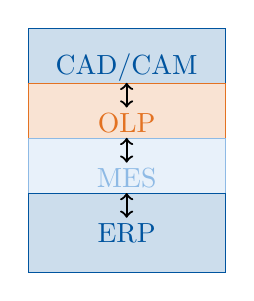
\begin{tikzpicture}[scale=0.7]
\node[draw,primary,fill=primary!20,minimum width=2.5cm,minimum height=1cm,align=center] (cad) at (0,3) {CAD/CAM};
\node[draw,accent,fill=accent!20,minimum width=2.5cm,minimum height=1cm,align=center] (olp) at (0,2) {OLP};
\node[draw,secondary,fill=secondary!20,minimum width=2.5cm,minimum height=1cm,align=center] (mes) at (0,1) {MES};
\node[draw,primary,fill=primary!20,minimum width=2.5cm,minimum height=1cm,align=center] (erp) at (0,0) {ERP};
\draw[<->,thick] (cad) -- (olp);
\draw[<->,thick] (olp) -- (mes);
\draw[<->,thick] (mes) -- (erp);
\end{tikzpicture}
\end{center}
\end{column}
\end{columns}

\vspace{0.5cm}
\begin{block}{Digital Twin Concept}
\begin{itemize}
\item \textbf{Virtual replica}: Real-time synchronization
\item \textbf{Predictive analytics}: Performance forecasting
\item \textbf{Continuous optimization}: Real-time adjustments
\item \textbf{Remote monitoring}: Cloud-based access
\end{itemize}
\end{block}
\end{frame}

\begin{frame}{Future Trends in Robot Programming Systems}
\begin{columns}[T]
\begin{column}{0.5\textwidth}
\begin{block}{Technical Trends}
\begin{itemize}
\item \textbf{Cloud-based OLP}: Remote simulation
\item \textbf{AI-powered programming}: Automatic optimization
\item \textbf{Virtual/Augmented Reality}: Immersive programming
\item \textbf{Natural language}: Voice/gesture control
\item \textbf{Blockchain}: Secure program distribution
\item \textbf{Edge computing}: Distributed processing
\end{itemize}
\end{block}
\begin{alertblock}{Industry 4.0 Integration}
\begin{itemize}
\item \textbf{IoT connectivity}: Sensor data integration
\item \textbf{Big data analytics}: Performance optimization
\item \textbf{Cyber-physical systems}: Seamless integration
\item \textbf{Smart factories}: Adaptive manufacturing
\end{itemize}
\end{alertblock}
\end{column}
\begin{column}{0.5\textwidth}
\begin{block}{Research Directions}
\begin{itemize}
\item \textbf{Automatic program synthesis}: From task description
\item \textbf{Learning from demonstration}: Imitation learning
\item \textbf{Collaborative programming}: Human-robot teams
\item \textbf{Adaptive programming}: Self-modifying code
\item \textbf{Explainable AI}: Understandable decisions
\end{itemize}
\end{block}
\begin{center}
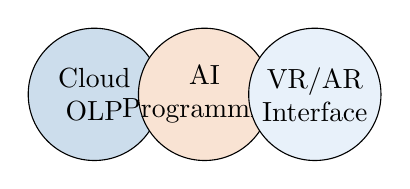
\begin{tikzpicture}[scale=0.7]
\draw[fill=primary!20] (0,0) circle (1.2);
\node[align=center] at (0,0) {Cloud\\OLP};
\draw[fill=accent!20] (2,0) circle (1.2);
\node[align=center] at (2,0) {AI\\Programming};
\draw[fill=secondary!20] (4,0) circle (1.2);
\node[align=center] at (4,0) {VR/AR\\Interface};
\end{tikzpicture}
\end{center}
\end{column}
\end{columns}
\end{frame}

\begin{frame}{Summary and Key Takeaways}
\begin{columns}[T]
\begin{column}{0.5\textwidth}
\begin{block}{Chapter 12: Robot Programming Languages}
\begin{itemize}
\item Specialized languages needed for unique robot requirements
\item Three generations: Motion-oriented $\rightarrow$ Structured $\rightarrow$ Task-oriented
\item Key features: Motion control, sensor integration, concurrency
\item Modern trend: Graphical, intuitive, cross-platform
\item Current standard: Vendor-specific but moving toward openness
\end{itemize}
\end{block}
\end{column}
\begin{column}{0.5\textwidth}
\begin{block}{Chapter 13: Off-line Programming Systems}
\begin{itemize}
\item Essential for complex tasks and reduced downtime
\item Core components: Modeling, planning, simulation, code generation
\item Critical issue: Calibration and accuracy requirements
\item Major benefit: Safety and optimization capabilities
\item Future direction: Cloud-based, AI-powered, integrated systems
\end{itemize}
\end{block}
\end{column}
\end{columns}

\vspace{1cm}
\begin{alertblock}{The Evolution of Robot Programming}
From \textbf{manual teach pendants} to \textbf{off-line simulation systems} to \textbf{AI-powered automatic programming}, the field continues to evolve toward more intuitive, efficient, and powerful tools for robot control and coordination.
\end{alertblock}
\end{frame}

\begin{frame}
\centering
\vspace{1cm}
{\Huge \textcolor{primary}{Thank You}}\\
\vspace{1cm}
{\Large Questions \& Discussion}\\
\vspace{2cm}
{\small Based on Craig, J.J. (2005). Introduction to Robotics: Mechanics and Control}\\
{\small Chapters 12 \& 13: Robot Programming Languages and Systems}\\
\vspace{0.5cm}
{\tiny Next: Chapter 14 - Force Control and Compliant Motion}
\end{frame}

\end{document}